%%%%%%%%%%%%%%%%%%%%%%%%%%%%%%%%%%%%%%%%%%%%%%%%%%%%%%%%%%%%%%%%%%%%%%%%%%%%%%
%
% PRÉAMBULE
%
%

% LaTeX 2e sinon rien !
\NeedsTeXFormat{LaTeX2e}

% C'est un rapport...
\documentclass[a4paper,11pt]{report}

% Style du document : personnalisé si disponible, sinon LaTeX par défaut
\newif\ifbglstyle
\IfFileExists{bglstyle.sty}{
  \usepackage{bglstyle} % Mon identité visuelle ;-)
  \bglstyletrue
}{
  \bglstylefalse
}

\ifbglstyle\else
  % Packages de base
  \usepackage[utf8]{inputenc}
  \usepackage[T1]{fontenc}
  \usepackage{ifpdf,textcomp,ae,aecompl,aeguill}
  \usepackage[margin=3cm]{geometry}

  % Commandes définies ici pour assurer la compatibilité avec le style perso
  \makeatletter
  \renewcommand{\title}[1]{\renewcommand{\@mytitle}{#1}}
  \newcommand{\@mytitle}{}
  \newcommand{\subtitle}[1]{\renewcommand{\@title}{\@mytitle\\#1}}
  \newcommand{\group}[1]{}
  \newcommand{\entity}[1]{}
  \makeatother

  % Si jamais le rendu du style LaTeX standard diffère légèrement du style
  % personnalisé, ça ne produira pas d'avertissement (overful/underful hbox)
  \sloppy
\fi

% Packages supplémentaires utilisés par ce document
\usepackage{graphicx,multicol}
\usepackage[french,english]{babel}

% Informations sur le document
\title{Résolveur parallèle type IDA* de (N²-1)-puzzles en UPC}
\author{Benjamin Gaillard, Lionel Imbs}
\date{2 mai 2006}
\group{Master 1 RIA --- Option IPP}
\entity{
\includegraphics[keepaspectratio,height=1.5cm]{images/ulp}}

% Hyperlinks
\ifpdf
  \usepackage[pdftex,bookmarks,bookmarksopen,bookmarksnumbered,%
              pdfstartview=Fit,pdfview=FitH]{hyperref}
  \makeatletter
  \hypersetup{%
    pdftitle  = {\@title},
    pdfauthor = {\@author},
    pdfborder = {0 0 0}
  }
  \makeatother
  \usepackage{thumbpdf}
\else
  \usepackage[dvips]{hyperref}
\fi

% Redéfinition d'une information (pour la présentation)
\title{%
{\large Introduction à la Programmation Parallèle}\\
  Résolveur parallèle type IDA*\\de (N\up{2} -- 1)-puzzles en UPC%
}
\subtitle{Rapport}
\author{Benjamin \textsc{Gaillard}\\Lionel \textsc{Imbs}}

% Commandes personnalisées
\newcommand{\ensp}[1]{\selectlanguage{english}#1\selectlanguage{french}}
\newcommand{\strong}[1]{\textbf{#1}}
\newcommand{\file}[1]{\ensp{\textsf{#1}}}
\newcommand{\var}[1]{\ensp{\textit{#1}}}
\newcommand{\type}[1]{\ensp{\texttt{#1}}}
\newcommand{\func}[1]{\ensp{\textsf{#1}}}
\newcommand{\class}[1]{\ensp{\textsf{#1}}}
\newcommand{\bs}{\textbackslash}

% Commandes pour ce rapport
\newcommand{\puz}{\emph{PuZ}}


%%%%%%%%%%%%%%%%%%%%%%%%%%%%%%%%%%%%%%%%%%%%%%%%%%%%%%%%%%%%%%%%%%%%%%%%%%%%%%
%
% CONTENU (enfin !)
%
%

\begin{document} % Pas d'indentation pour cet environnement de base

\selectlanguage{french}
\maketitle
\tableofcontents

\chapter*{Introduction}
\markboth{Introduction}{Introduction}
\addcontentsline{toc}{chapter}{Introduction}

Le but de ce projet est d'implémenter un programme parallèle de résolution de
$(N^2 - 1)$-puzzles en utilisant un algorithme de recherche en profondeur A*
(algorithme de plus court chemin de Dijkstra avec une heuristique). Le langage
utilisé est UPC, une extension du langage C permettant d'utiliser des
variables réparties sur plusieurs threads ainsi que des instructions
spécifiques aux systèmes parallèles.

Dans ce rapport nous allons décrire notre programme, appelé \puz, son
fonctionnement, les choix d'implémentation qui ont été faits puis nous allons
finalement étudier son efficacité en fonction du nombre de processeurs en
examinant des mesures de temps prises sur quelques exécutions.


\chapter{Organisation}

\noindent
Les sources du projet sont organisées de la manière suivante :
\begin{itemize}
  \item le répertoire \file{doc} contient la documentation, c'est-à-dire le
	sujet, le manuel d'UPC et le rapport ;
  \item le répertoire \file{matrices} contient quelques matrices sur
	lesquelles ont été effectués les tests ;
  \item le script \file{batch.sh}, utilisé pour lancer des exécutions en série
	pour tester le projet suivant un nombre différent de processeurs ;
  \item \file{common.h} : macros et définitions globales, communes à tous les
	fichiers ;
  \item \file{ida.h} : l'en-tête (interface) utilisé pour les deux
	implémentations de l'algorithme IDA* ;
  \item \file{ida-prl.upc} : la version parallèle de l'implémentation de
	l'algorithme IDA* (\emph{Iterative Deepening A*}) ;
  \item \file{ida-seq.c} : la version séquencielle de l'implémentation de
	l'algorithme IDA*, pour un seul processeur ;
  \item \file{input.c} et \file{input.h} : les fonctions de lecture des
	matrices ;
  \item \file{main.c} : la fonction principale du programme, qui lit les
	paramètres passés à l'exécutable, procède aux initialisations et
	appelle les autres fonctions ;
  \item \file{util.c} et \file{util.h} : fonctions utilitaires utilisées par
	les deux implémentations de l'algorithme IDA* (calcul de l'heuristique
	de Manhattan, exécution d'un mouvement sur la matrice, retour en
	arrière d'un mouvement, etc.).
\end{itemize}

\paragraph{Note} Le fichier \file{Makefile} peut être modifié en fonction de
l'environnement et du compilateur utilisés. Il a été testé avec GCC, le
compilateur Intel C++ et Microsoft Visual C++\footnote{Disponible gratuitement
sous l'intitulé \og Microsoft Visual C++ Toolkit 2003\fg} (avec Wine) pour son
implémentation en C et avec GCC-UPC et Berkeley UPC/Intel C++ pour sa version
UPC.


\chapter{Langages}

\section{Deux versions}

Deux implémentations de \puz{} ont été effectuées : une version séquencielle,
prévue pour s'exécuter sur un seul processeur et une version parallèle
pouvant être lancée sur une architecture à plusieurs processeurs.

La version séquencielle est écrite en C et peut donc être compilée avec
n'importe quel compilateur. Le type \type{bool} de C99 est utilisé, mais si le
compilateur ne supporte pas cette norme (compilateur ANSI C/ISO C/C89/C90) le
type \type{unsigned char} est automatiquement utilisé à la place.

L'implémentation parallèle est écrite en langage
\href{http://upc.gwu.edu/}{UPC (\emph{Unified Parallel C})} et est donc
compilable avec une implémentation de ce langage. \puz{} a été testé avec
\href{http://upc.nersc.gov/}{Berkeley UPC} (le compilateur présent sur la
machine \emph{hpc}) et \href{http://www.intrepid.com/upc/}{GCC-UPC}, un patch
pour \href{http://gcc.gnu.org/}{GCC} développé par
\href{http://www.intrepid.com/}{Intrepid.com}.

Pour les besoins du projet, un \emph{ebuild} a été créé pour installer GCC-UPC
sur une distribution \href{http://www.gentoo.org/}{Gentoo Linux}. Il a été
envoyé sur le \href{http://bugs.gentoo.org/}{Bugzilla de Gentoo} et est en
attente d'un mainteneur pour intégration dans l'arbre Portage officiel. Le
rapport de bug correspondant est disponible à cette adresse :
\href{http://bugs.gentoo.org/show_bug.cgi?id=130388}
{\sffamily\ensp{http://bugs.gentoo.org/show\_bug.cgi?id=130388}}.

\section{Différences d'implémentation entre les langages}

Pour des raisons de simplicité et de rapidité, nous avons développé \puz{} en
local sur nos machines en utilisant GCC-UPC. Cela nous a grandement aidé,
cependant nous avons éprouvé quelques difficultés à faire fonctionner notre
programme avec Berkeley UPC à cause de certaines différences d'implémentation
entre les deux compilateurs.

Il existe des différences notoires entre GCC-UPC et Berkeley UPC : en effet,
GCC-UPC est prévu pour fonctionner sur une architecture SMP, où chaque
processeur partage donc la mémoire centrale avec tous les autres. Il n'y a pas
de passage de message dans cette implémentation. Berkeley UPC, au contraire,
est capable de tourner dans un environnement où les processeurs sont situés
sur des machines différentes et doit donc envoyer des messages pour la
communication entre les \emph{threads}.

La différence principale est que les écritures sont immédiatement répercutées
avec GCC-UPC. Si l'on utilise Berkeley UPC, on doit appeler des fonctions UPC
pour que les messages soient émis et, surtout, que les messages entrant soient
lus. La lecture de variables n'est pas concernée car cette action est
synchrone.

La principale répercussion de ce \og problème\fg{} est que les \emph{threads}
qui ne font que des traitements locaux vont ignorer les messages entrant et
donc bloquer les \emph{threads} qui dépendent des réponses à ces messages pour
continuer leur exécution. Par exemple, une attente active de type \og%
\verb+while (!var);+\fg{} provoquera des blocages.

\bigskip\noindent
Pour y remédier, nous disposons des moyens suivants :
\begin{itemize}
  \item l'instruction \verb!upc_barrier! lorsque cela est approprié : celle-ci
	traite les messages en attendant que tous les \emph{threads} soient
	synchronisés ;
  \item l'instruction \verb!upc_fence! qui sert à traiter tous les messages
	dans les tampons d'entrée et éventuellement de sortie (mode relaxé) ;
  \item utiliser des variables de type \type{strict} : cela revient au même
	que d'utiliser des variables de type \type{relaxed} (par défaut) et
	d'appeler \verb!upc_fence! avant et après les accès à ces variables.
\end{itemize}

\bigskip
Une solution concernant l'exemple évoqué plus haut est de réécrire la boucle
de la façon suivante : \og\verb+while (!var) upc_fence;+\fg. Une autre serait
de déclarer la variable \var{var} d'un type \type{strict}.

\section{Optimisation des performances}

Afin d'atteindre des performances optimales, nous avons effectué certaines
optimisations sur notre programme.

Tout d'abord, les variables partagées régulièrement scrutées tout au long de
l'exécution de l'application ont été transformées en pointeurs locaux de type
\type{volatile}. Cela nous permet d'éviter la conversion d'adresse partagée
en adresse qui sera de toute façon locale. Nous économisons donc un peu de
temps. Nous éliminons la mise en cache par le compilateur de ces variables en
les déclarant \type{volatile}, au cas où elles seraient modifiées par un autre
\emph{thread}.

\section{Débogage et qualité}

Afin de pouvoir déboguer plus aisément notre projet et d'en assurer la
meilleure qualité possible, au début de chaque fonction, ses paramètres sont
testés (assertions) au moyen de la macro \func{assert()}. Des assertions sont
aussi présentes dans le code de certaines fonctions quand cela est approprié.

De plus, nous avons pris soit de documenter chaque fonction dans un style
Doxygen. Des commentaires ont également été placés un peu partout dans le code
pour permettre une compréhension optimale de notre programme.


\chapter{Implémentation}

\section{Privilège des traitements locaux}

Les traitements locaux sont favorisés par rapport aux traitements distants et
aux envois de messages. Tout a donc été fait pour qu'il y aît un minimum de
communication entre les threads pour optimiser au mieux les performances. Si
quelque chose peut être fait localement, cette méthode est priviligiée.

\section{Une valeur par thread}

Dans plusieurs cas, il était nécessaire que chaque thread possède sa propre
valeur pour une variable. C'est le cas, par exemple, du poids pour
l'algorithme de terminaison en arbre, du jeton possédé (ou pas) par un
processeur pour l'algorithme de terminaison Dijkstra modifié, des verrous pour
la distribution de travail, la valeur minimale de l'heuristique des feuilles
de l'arbre parcouru\dots

Dans la quasi totalité des cas, un pointeur vers la variable correspondant au
thread en cours est utilisé, cela nous évitant de faire la conversion depuis
un pointeur vers donnée partagée à chaque fois. Au final, c'est donc plus
performant.

Par exemple, pour un tableau déclaré ainsi : \og%
\verb!shared int all_tab[THREADS];!\fg, nous déclarons un pointeur \og%
\verb!volatile int *my_tab;!\fg{} auquel nous affectons la valeur \og%
\verb!(int *) all_tab[MYTHREAD]!\fg. Par la suite, nous accéderons toujours à
la valeur concernant notre thread au moyen du pointeur \var{my\_tab} qui se
fera directement, sans conversion.

\section{Obtention de travail}

\subsection{Choix du donneur}

Les trois algorithmes du choix du donneur ont été implémentés. L'algorithme
cyclique global utilise un verrou pour garantir une exclusion mutuelle sur
la variable contenant le numéro du donneur. Il est ainsi garanti que deux
threads ne demandent pas de travail au même thread au même instant donné
exactement (il est cependant possible que cela arrive dans de rares cas où
cette variable a \og fait un tour\fg{} complet et qu'un thread demandeur n'a
toujours pas reçu son travail).

Les autres méthodes ont un traitement entièrement local, il n'est donc point
besoin de les étudier au vu de leur trivialité. À noter qu'à chaque itération
de la boucle principale de l'algorithme IDA*, l'initiateur (le thread 0)
débute le traitement sur un nouveau chemin, sans en demander aux autres. Les
autres threads demanderont donc en premier à l'initiateur de donner du
travail. Une fois le premier travail de l'initiateur accompli, celui-ci va
en demander à un autre thread, comme tous les autres.

\subsection{Transmission du travail}

Chaque thread possède son propre \og chemin\fg{} qui correspond aux directions
prises depuis l'état initial. Ce chemin se situe dans la zone partagée d'un
thread mais qui a une affinité avec celui-ci. Cette zone de mémoire est donc
traitée comme de la mémoire privée lors de l'exécution, ce qui ne pénalise pas
le programme du point de vue des performances. Cette mémoire est allouée
dynamiquement à chaque itération de la boucle principale de l'algorithme IDA*,
c'est-à-dire quand la limite change. Nous allons appeler cette zone de mémoire
\var{path}.

Chaque thread possède également deux autres variables : une indiquant la
longueur du chemin transmis (\var{length}), l'autre l'identifiant d'un
éventuel demandeur de travail (\var{worker}). De plus, chaque thread a accès à
un tableau partagé de verrous (\var{lock}), un pour chaque thread.

\bigskip
Voici ce qui se passe lorsqu'un thread demande du travail à un autre (ceci est
du pseudo code, le chemin n'est pas copié comme cela) :

\begin{table}[!htb]
  \centering
  \begin{tabular}{|l||l|}
    \hline
    \multicolumn{1}{|c||}{\textbf{Fournisseur (\var{provider})}} &
    \multicolumn{1}{c|}{\textbf{Demandeur (\var{seeker})}}\\
    \hline\hline
    \verb+worker[provider] = provider;+ &\\
    \hline\hline
    & \verb+lock(lock[provider]);+\\
    & \verb+length[seeker] = -1;+\\
    & \verb+worker[provider] = seeker;+\\
    & \verb+while (length[seeker] == -1);+\\
    \hline
    \verb+seeker = worker[provider];+ &\\
    \verb+if (seeker == provider) return;+ &\\
    \verb+worker[provider] = provider;+ &\\
    \verb+path[seeker] = path[provider];+ &\\
    \verb+length[seeker] = path_length;+ &\\
    \hline
    & \verb+unlock(lock[provider]);+\\
    \hline
  \end{tabular}
  \caption{Algorithme de transmission du travail}
\end{table}

\bigskip
Cette méthode nous permet de faire un usage minimal des ressources partagées
avec tous les autres threads, ce qui entraîne des performances optimales. On
ne perd pas de temps, à part lors de l'attente active. Mais cela de pose pas
de problème puisque de toute façon le thread n'a pas de travail à cet instant.

En résumé, nous utilisons un verrou uniquement, ce qui est le minimum
nécessaire pour que deux threads ne demandent pas en même temps du travail au
même thread, mais qu'ils le fassent chacun leur tour. Toutes les autres
communications se font directement entre le fournisseur et le demandeur de
travail.

\section{Détection de la terminaison}

Il est nécessaire de pouvoir détecter la terminaison d'une itération de la
boucle principale de l'algorithme IDA*, autrement dit quand plus aucun thread
n'a de travail. Trois algorithmes ont été implémentés à cette fin : les deux
proposés dans le sujet ainsi qu'un algorithme supplémentaire qui nous a paru
bien plus simple et plus performant.

Chaque thread possède une variable \var{term} qui peut prendre trois valeurs :
\begin{itemize}
  \item \var{working} : le thread est en train de travailler ;
  \item \var{end} : le thread a terminé son travail et en cherche un nouveau ;
  \item \var{found} : une solution a été trouvée.
\end{itemize}

Pour optimiser les performances, chaque thread ne va pas tester lui-même la
condition de terminaison à chaque fois. Au lieu de cela, un seul thread va
tester, à des moments stratégiques (à la fin d'un travail par exemple) en
fonction de la méthode choisie, si la terminaison est atteinte. Si c'est le
cas, il va modifier la variable \var{term} de tous les threads en y mettant la
valeur \var{end}.

Dans le cas où une solution a été trouvée, il s'agit à peu près de la même
chose : le thread qui a trouvé une solution va mettre la valeur \var{found}
dans la variable \var{term} de tous les threads.

Ainsi, chaque thread n'aura qu'à tester continuellement sa propre variable
\var{term} pour vérifier si la condition de terminaison a été atteinte. Un
minimum de communication entre les threads est alors assuré, pour des
performances optimales.

Le cas spécial dans lequel une solution est trouvée est traité à part. Si
cette condition est vérifiée, chaque thread termine immédiatement son
exécution, même s'il est en train d'effectuer un travail. Puisqu'il est
certain que la première solution trouvée sera optimale (ce n'est pas forcément
la seule cependant), il n'est plus utile de poursuivre l'exécution du
programme.

\subsection{Algorithme de Dijkstra modifié}

Les threads se passent le jeton en mettant à jour leur couleur et celle du
jeton exactement comme indiqué dans le sujet. Chaque thread, lorsqu'il est
inactif, scrute continuellement sa propre variable pour savoir s'il possède le
jeton et le transmettre le cas échéant. L'initiateur est chargé de détecter
la terminaison.

\subsection{Algorithme de l'arbre}

L'implémentation suit les indications du sujet. Lorsqu'un thread est inactif,
il vérifie son poids, et s'il n'est pas nul, le transmet à son parent. Un
verrou est ici utilisé pour que deux threads ne donnent pas leur poids en
même temps. L'initiateur est chargé de détecter la terminaison qui se produit
lorsque son poids est revenu à 1.

\subsection{Algorithme supplémentaire : le compteur}

Un compteur global est initialisé à 1 à chaque itération de la boucle
principale de l'algorithme IDA*. Quand un thread reçoit du travail d'un
autre thread (ce qui exclue donc l'initiateur qui commence un nouveau
travail), il incrémente cette variable; quand son travail est terminé, il la
décrémente. L'accès à cette variable est protégée par un verrou pour que deux
threads n'y accèdent pas au même instant.

La détection de terminaison est effectuée par chaque thread lorsqu'il a fini
son travail. Si le compteur est nul à ce moment-là, il communique aux autres
threads que la terminaison a été atteinte.

\section{Compilation et exécution du programme}

\puz{} est compilé en lançant \verb!make! dans le répertoire contenant les
sources. Il y aura peut-être besoin d'adapter le fichier \file{Makefile}
suivant l'environnement de compilation.

Il est possible de passer des options à l'exécutable, permettant entre autres
de spécifier l'algorithme de sélection du donneur et celui de détection de
terminaison. On peut aussi indiquer un fichier d'entrée et/ou de sortie.
D'autres options sont également disponibles.

Pour avoir une liste descriptive de ces options, il suffit de lancer le
programme avec l'option \og\verb!-h!\fg. À noter que la version parallèle
dispose évidemment de plus d'options que la version séquencielle.


\chapter{Mesures de performance}

\section{Importance de la distribution du travail}

Comme tous les threads arrêtent leur exécution dès qu'une solution a été
trouvée, la durée totale d'exécution est très dépendante de la façon dont est
distribué le travail entre les threads. Pour illustrer ceci, nous allons
examiner un exemple d'exécution du programme.

Nous allons étudier le cas suivant, où trois threads sont en exécution. Le
premier, l'initiateur, part de la racine. Il est important de noter que les
threads donnent toujours comme travail l'état non développé le plus proche de
la racine, et qu'ils parcourent l'arbre toujours dans le même ordre, de gauche
à droite.

\begin{figure}[!htb]
  \centering\bigskip\noindent
  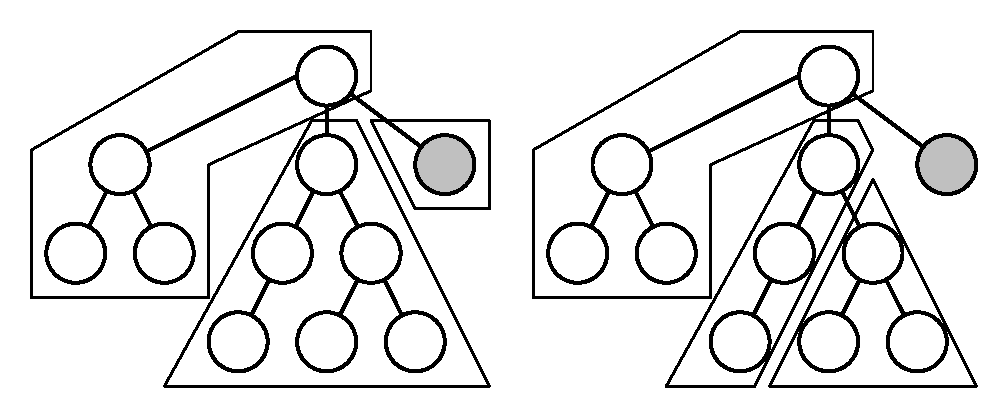
\includegraphics[keepaspectratio,width=.9\textwidth]{schemas/tree}
  \caption{Exemple de répartition du travail}
\end{figure}

\bigskip
Deux cas sont présentés ici. Dans le premier, les deux autres threads
demandent chacun du travail à l'initiateur. Dans le deuxième cas, le deuxième
thread demande du travail au premier, et le troisième au deuxième. Nous voyons
sur le schéma la distribution du travail par les \og boîtes\fg{} qui entourent
les n\oe uds de l'arbre. Le n\oe ud gris correspond à un état final.

Imaginons que le fait de tester un n\oe ud pour savoir s'il s'agit d'une
solution prenne énormément de temps (ou, tout simplement, que les arbres ne
sont ici pas développés et qu'ils ont une profondeur bien plus grande). Nous
pouvons en conclure que dans le premier cas l'exécution sera presque
instantanée puisque le troisième thread trouve tout de suite la solution.
Dans l'autre cas en revanche, la durée d'exécution sera bien plus longue.

Nous pouvons donc remarquer que la durée d'exécution totale du programme peut
grandement varier en fonction de la distribution du travail et qu'elle est
donc tributaire de l'algorithme de sélection du donneur ainsi que de l'ordre
dans lequel les threads vont effectuer leur demande.

Tout cela pour expliquer que certains variations, parfois assez grandes,
peuvent survenir dans les mesures de temps d'exécution. Cela n'a rien
d'anormal, c'est juste une conséquence des différents choix d'algorithme et
du hasard.

\section{Mesures de temps}

\noindent
Voici les mesures de temps effectuées sur deux matrices différentes :

\begin{table}[!htb]
  \centering
  \begin{tabular}{|r|r@{,}l|r@{,}l|}
    \hline
    \textbf{Processeurs} &
    \multicolumn{2}{c|}{\textbf{Temps cas 1 (s)}} &
    \multicolumn{2}{c|}{\textbf{Temps cas 2 (s)}}\\
    \hline\hline
     1 & 630&898 & 43&483\\
     2 & 176&728 & 12&597\\
     3 & 177&910 & 12&632\\
     4 & 176&690 & 12&600\\
     5 & 177&984 & 12&697\\
     6 & 178&100 & 12&694\\
     7 &   9&785 & 12&737\\
     8 &  29&911 & 12&607\\
     9 &   0&660 & 12&698\\
    10 &   9&779 & 12&757\\
    11 &   0&661 & 12&695\\
    12 &   0&662 & 12&728\\
    13 &   0&661 & 12&672\\
    14 &   0&661 &  5&664\\
    15 &   0&662 &  9&556\\
    16 &   0&657 &  5&654\\
    \hline
  \end{tabular}
  \caption{Mesures de temps d'exécution}
\end{table}

\section{Calcul des résultats}

Rappel des formules utilisées pour les calculs :

\noindent
$T_1(n)$ = temps nécessaire sur 1 processeur pour un problème de taille $n$.\\
$T_p(n)$ = temps nécessaire sur $p$ processeurs pour un problème de taille
$n$.

\bigskip\noindent
\[\textrm{Accélération (\emph{speed-up}) : } S(n, p) = \frac{T_1(n)}{T_p(n)}\]
\[\Rightarrow \textrm{Efficacité : } E(n, p) = \frac{S(n, p)}{p}\]

\noindent
A partir de nos mesures, nous obtenons les accélérations et efficacités
suivantes :

\begin{table}[!htb]
  \centering
  \begin{tabular}{|r|r@{,}l|r@{,}l|r@{,}l|r@{,}l|}
    \hline
    &
    \multicolumn{4}{c|}{\textbf{Cas 1}} &
    \multicolumn{4}{c|}{\textbf{Cas 2}}\\
    \hline
    \textbf{Processeurs} &
    \multicolumn{2}{c|}{\textbf{Accélération}} &
    \multicolumn{2}{c|}{\textbf{Efficacité}}   &
    \multicolumn{2}{c|}{\textbf{Accélération}} &
    \multicolumn{2}{c|}{\textbf{Efficacité}}\\
    \hline\hline
     1 &   1&000 &   1&000 & 1&000 & 1&000\\
     2 &   3&570 &   1&785 & 3&452 & 1&726\\
     3 &   3&546 &   1&182 & 3&442 & 1&147\\
     4 &   3&571 &   0&893 & 3&451 & 0&863\\
     5 &   3&545 &   0&709 & 3&425 & 0&685\\
     6 &   3&542 &   0&590 & 3&425 & 0&571\\
     7 &  64&476 &   9&211 & 3&414 & 0&488\\
     8 &  21&093 &   2&637 & 3&449 & 0&431\\
     9 & 955&906 & 106&212 & 3&424 & 0&380\\
    10 &  64&516 &   6&452 & 3&409 & 0&341\\
    11 & 954&460 &  86&769 & 3&425 & 0&311\\
    12 & 953&018 &  79&418 & 3&416 & 0&285\\
    13 & 954&460 &  73&420 & 3&431 & 0&264\\
    14 & 954&460 &  68&176 & 7&677 & 0&548\\
    15 & 953&018 &  63&535 & 4&550 & 0&303\\
    16 & 960&271 &  60&017 & 7&691 & 0&481\\
    \hline
  \end{tabular}
  \caption{Calcul des accélérations et des efficacités}
\end{table}

Ces différentes valeurs peuvent être représentées graphiquement pour une
compréhension et une interprétation plus aisées : voir figure \ref{graphes}.

\begin{figure}[!htb]
  \centering\noindent
  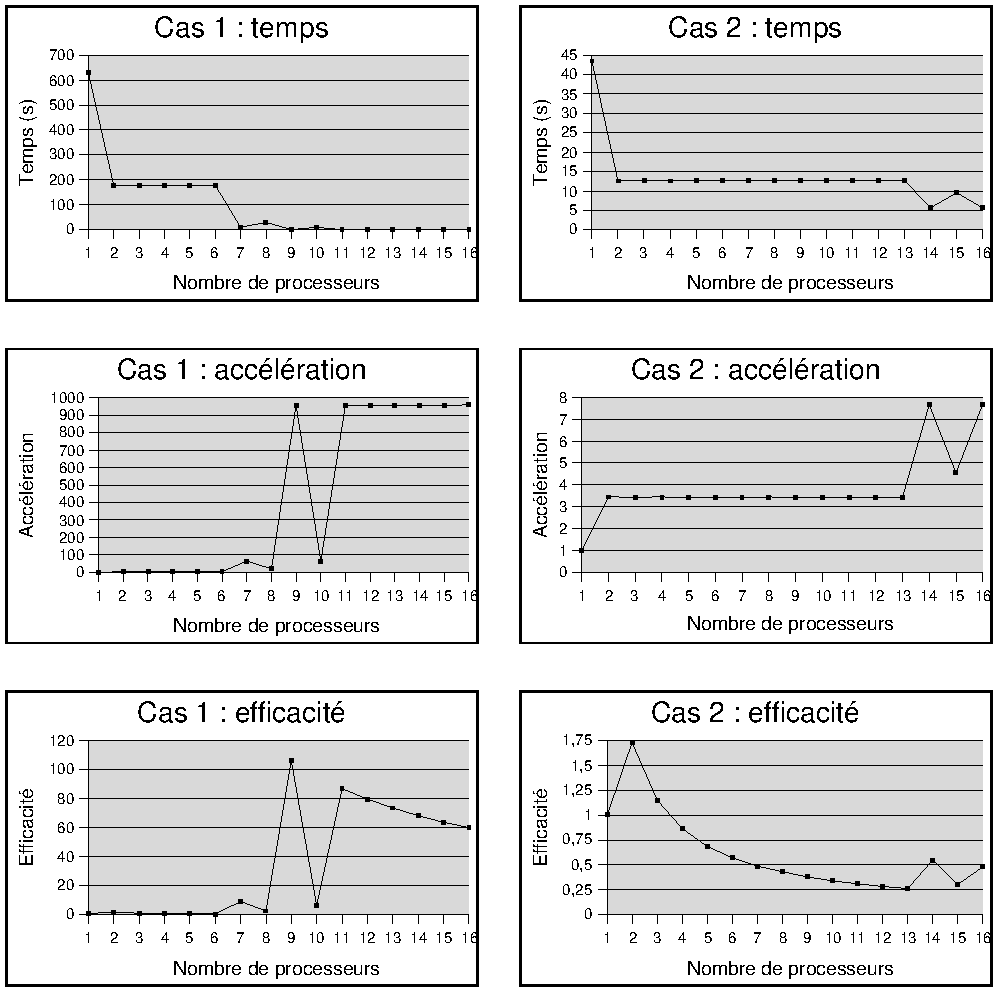
\includegraphics[keepaspectratio,width=\textwidth]{schemas/mesures}
  \caption{Graphes de temps, d'accélération et d'efficacité}
  \label{graphes}
\end{figure}

\section{Interprétation des résultats}

\subsection{Accélération}

Nous remarquons que l'augmentation du nombre de processeurs ne se traduit
rapidement plus par un gain de performance. Cette limite est causée par la
granularité de l'algorithme et par les aléas décrits plus haut.

\subsection{Efficacité}

Nous pouvons déduire de ces mesures que le nombre de processeurs où
l'efficacité maximale est atteinte est très variable suivant les jeux de
données. Dans le premier cas il est de 9, dans le second de 2. De même que
pour l'accélération, divers facteurs permettent éventuellement d'expliquer
ce comportement plutôt chaotique.

\subsection{Iso-efficacité}

Par définition, l'iso-efficacité définit une relation entre le nombre de
processeurs, la taille du problème et l'efficacité que l'on souhaite
atteindre.

Seulement, comme nous avons pu le voir grâce aux représentations graphiques
précédentes, il difficile de caractériser mathématiquement l'accélération en
fonction du nombre de processeurs. Ce postulat est directement lié à
l'algorithme utilisé. Nous ne pouvons donc déduire de nos mesures une relation
d'iso-efficacité.


\chapter*{Conclusion}
\markboth{Conclusion}{Conclusion}
\addcontentsline{toc}{chapter}{Conclusion}

Ce projet, bien plus complexe qu'il n'y paraît au premier abord, nous a permis
d'appliquer les principes fondamentaux d'UPC que nous avons pu étudier en
cours. À l'aide d'un exemple concret, nous avons pu mesurer le gain de
performances induit par la parallélisation d'un algorithme. Nous avons ainsi
tiré parti de la puissance d'un cluster en terme de calculs.

Les gains sont surprenants dès lors que l'on augmente le nombre de
processeurs. Le problème devient alors insignifiant face à l'efficacité du
traitement. Les gains sont tels que les heures de programmation ont été
compensées par les résultats.

\end{document}
